\chapter{Theoretische Grundlagen}

\section{magnetische Kernspinresonanz}

Atomkerne mit einem Kernspin $\vec I$ besitzen ein dem Kernspin proportionales magnetisches Dipolmoment $\vec
\mu_I$:
	\[
		\vec \mu_I=\gamma\,\vec I
	\]
Dabei ist $\gamma$ ist das gyromagnetische Verhältnis (von Spin und magnetischem Moment). Die
Einheit des magnetischen Kernmoments ist, in Analogie zum Bohrschen Magneton $\mu_B$ der
Elektronen, das Kernmagneton $\mu_K$, das um das Verhältnis von Elektronen"= zu Protonenmasse
kleiner als $\mu_B$ ist.
	\[
		\vec\mu_I=\frac{g_I\,\mu_K}{\hbar}\vec I,\ttextt{mit}\mu_K=0.505\cdot10^{-26}\text{Am}^2
	\]
Man kann weiterhin in Analogie zu den Elektronen einen Kern"=$g$"=Faktor einführen, der durch
$g_I=(\gamma\;\hbar/\mu_K)$ definiert ist. Allerdings ergibt sich $g_I$ im Gegensatz zum
Landé"=$g_J$"=Faktor der Elektronenschalen nicht aus den das System beschreibenden
Quantenzahlen, sondern ist eine empirische, für jedes Nukleon charakteristische Meßgröße.

Für den Betrag des Drehimpulses des Kerns gilt:
	\[
		\abs{\vec I}=\sqrt{I(I+1)}\;\hbar
	\]
Die so definierte Kernspinquantenzahl $I$ ist ganz oder halbzahlig.

Meßbar ist nur die Komponente von Spin und magnetischem Moment in der Vorzugsrichtung, die durch
die Richtung eines von außen angelegten Magnetfeldes $\vec B_0$ vorgegeben ist. Im Weiteren ist
die Richtung der $z$"=Achse im Koordinatensystem immer durch diese Vorzugsrichtung festgelegt. Für
die Komponenten von Kernspin und magnetischem Moment parallel zu dieser Vorzugsrichtung gilt
dann:
	\[
		I_z = m_I\;\hbar\ttextt{und}\mu_z=\gamma\;\hbar m_I=g_I\mu_Km_I
	\]
Hierbei ist $m_I$ die magnetische Quantenzahl des Kernspins. Sie kann Werte im Intervall $[-I,
-I+1, \ldots, I-1, I]$ annehmen und repräsentiert die $(2I+1)$"=fache Möglichkeit der Einstellung
der $z$"=Komponente des Kernspins relativ zur Vorzugsrichtung. Die Vorzeichen des magnetischen
Moments $\vec\mu_I$ und des $g_I$"=Faktors können positiv oder negativ sein.

In einem äußeren Magnetfeld $\vec B_0$ besitzt ein Kern aufgrund seines magnetischen Moments die
magnetische Wechselwirkungsenergie (Zeemann"=Energie)
	\[
		V=-\vec \mu_I\cdot\vec B_0=-g_I\,\mu_K\,B_0\,m_I\ttext{.}
	\]
Diese äquidistanten Energieniveaus sind im thermischen Gleichgewicht nach der Boltzmannverteilung
\eqref{eqn:boltzmann} besetzt. Die Energiedifferenz zwischen zwei benachbarten
Einstellmöglichkeiten des magnetischen Moments im Feld $\vec B_0$ und damit die Energie für Dipolübergänge
mit $\Delta m_I=\pm1$, beträgt demnach
	\[
		\Delta E=g_I\,\mu_K\,B_0\ttext{.}
	\]
Strahlt man auf eine Probe, senkrecht zu $\vec B_0$ elektromagnetische Wellen ein, die die
Resonanzbedingung
	\begin{equation}
		\label{eqn:resonanzbed}
		\omega=\frac{\Delta E}{\hbar}=\frac{g_I\,\mu_K}{\hbar}B_0
	\end{equation}
erfüllen, so kann diese Strahlung von der Probe absorbiert werden und somit magnetische
Dipolübergänge zwischen den möglichen Kernspin"=Orientierungen induzieren. Diesen Prozeß nennt man
Kernspin"=Resonanz. Diese Resonanz bedeutet ein Übereinstimmen der Frequenz der eingestrahlten
Strahlung mit der Larmor"=Präzessionsfrequenz, mit der die Kernspins im Magnetfeld $\vec B_0$ um
dessen Richtung präzedieren.

Der Vorteil der Resonanzmethode besteht darin, daß der Anteil der Kernsuszeptibilität an der
Gesamtsuszeptibilität selektiv betrachtet werden kann, auch wenn ihr Beitrag relativ klein ist.
Zusätzlich liefert die NMR aus den meßbaren Relaxationszeiten Informationen über
Wechselwirkungsprozesse, die auf atomarem Niveau ablaufen.

Man unterscheidet zwei Methoden der Bestimmung von NMR"=Spektren:
	\begin{itemize}
		\item Eine Möglichkeit, NMR"=Spektren aufzunehmen, ist die Methode der
			\emph{cw"=Kernspinresonanz} (cw = \ul{c}ontinuous
			\ul{w}ave). Hierbei wird über die Probenspule ständig ein schwaches Hochfrequenzsignal
			eingestrahlt. Man kann nun entweder die Frequenz des schwachen Hochfrequenzsignals
			langsam ändern oder durch Änderung der Stärke des äußeren Feldes $B_0$ nach Gleichung 
			\eqref{eqn:resonanzbed} die NMR"=Resonanzfrequenzen relativ zur eingestrahlten Frequenz
			verändern. Das Resonanzspektrum wird durch Messung der
			Energieabsorption in der NMR"=Spule in Abhängigkeit von der angeregten Frequenz oder
			der Magnetfeldstärke aufgenommen.
		\item Für die Messungen im Rahmen dieser Arbeit wurde die Methode der \emph{gepulsten
			Kernspinresonanz} verwendet. Hierbei wird senkrecht zum Feld $\vec B_0$ ein Hochfrequenzpuls
			der Amplitude $B_\mathrm{HF}$ für die Zeit $t_\mathrm{Puls}$ mit Hilfe einer Spule in die Probe eingestrahlt
			(siehe dazu auch Abb.~\ref{fig:probe} auf Seite~\pageref{fig:probe}).
			Nach Pulsende verwendet man dieselbe Probenspule dazu, um Änderungen
			des magnetischen Flusses in Spulenrichtung zu detektieren. Nach dem HF"=Puls erhält man
			eine makroskopisch meßbare Komponente der Probenmagnetisierung senkrecht zu $\vec
			B_0$. Die makroskopische Magnetisierung präzediert somit mit der Larmorfrequenz um die
			Richtung von $\vec B_0$. Das führt dazu, daß sich der magnetische Fluß durch die
			Probenspule periodisch ändert. Die in der Probenspule induzierte Spannung ist somit
			proportional zur Änderung des magnetischen Flusses in Spulenrichtung. Dieses Signal,
			daß proportional zur zeitlichen Änderung der Probenmagnetisierung in Spulenrichtung
			ist, nennt man den freien Induktionszerfall (auch \ul{f}ree \ul{i}nduction \ul{d}ecay,
			{\bfseries FID}). Das NMR"=Resonanzspektrum kann man durch Fouriertransformation aus
			dem aufgezeichneten FID ermitteln.
	\end{itemize}

Als Modell für die \emph{gepulste Kernspinresonanz} kann man die Schrödingergleichung für
einen freien Spin $I=\frac12$ in einem konstanten Magnetfeld $\vec B_0$ und einem schwachen dazu
senkrechten zeitabhängigen Magnetfeld lösen.
Dieses zeitabhängige Magnetfeld rotiert mit der Amplitude $B_\mathrm{HF}$ und der Larmorfrequenz
$\omega_0=\frac{g_I\mu_KB_z^0}{\hbar}$ in der $xy$"=Ebene. Die Schrödingergleichung lautet dann:
	\begin{equation}
		\left(-\vec\mu\cdot{\vec B}\right) \phi = i\;\hbar \frac{d\phi}{dt}
	\end{equation}
mit
	\[
			\vec B= \begin{pmatrix}0\\0\\B_z^0\end{pmatrix}+
					\begin{pmatrix}B_x^s(t)\\B_y^s(t)\\0\end{pmatrix}
	\ttextt{und}
		\begin{matrix}
			B_x^s(t) = B_\mathrm{HF}\cos(\omega_0t)\\ 
			B_y^s(t) = B_\mathrm{HF}\sin(\omega_0t)
		\end{matrix}
	\]
Mit $\Omega=\frac{\mu_I\mu_K}{\hbar}B_\mathrm{HF}$ kann man nun die zeitliche Entwicklung der
Erwartungswerte der Spinkomponenten und somit auch der des magnetischen Moments herleiten:
	\begin{equation}
		\label{eqn:s_xyz}
		\begin{array}{rl}
			\left<\mu_x\right>&=-\frac{\gamma\;\hbar}2\sin(\Omega t)\sin(\omega_0t)\\
			\left<\mu_y\right>&=\phantom{-}\frac{\gamma\;\hbar}2\sin(\Omega t)\cos(\omega_0t)\\
			\left<\mu_z\right>&=-\frac{\gamma\;\hbar}2\cos(\Omega t)
		\end{array}
	\end{equation}
Wie man sieht, beschreiben $\cos(\Omega t)$ und $\sin(\Omega t)$ die Auslenkung der
Gleichgewichtsmagnetisierung aus der z"=Richtung, den sog.\ \emph{Tippingwinkel} $\theta$. Dieser ist
danach proportional zum Produkt aus der Amplitude und der Zeitdauer des HF"=Pulses:
	\begin{equation}
		\theta_\mathrm{tip} = \Omega t_\mathrm{Puls}
			= \frac{\mu_I\mu_K}{\hbar}B_\mathrm{HF}t_\mathrm{Puls}
	\end{equation}
Die Terme $\sin(\omega_0t)$ und $\cos(\omega_0t)$ beschreiben die Larmorpräzession des
magnetischen Moments in der $xy$"=Ebene.

Wenn man die Zeitableitung der Gleichungen \eqref{eqn:s_xyz} bildet, erhält man die
Bewegungsgleichung für die Erwartungswerte des magnetischen Moments:
	\begin{equation}
		\frac{d}{dt}\left<\vec \mu\right>=\gamma\left<\vec\mu\right> \times \vec B(t)\ttext{.}
	\end{equation}

Diese Gleichung, die für eine beliebige Zeitabhängigkeit des Magnetfeldes $\vec B(t)$ gültig
ist, erinnert an die Kreiselgleichung der klassischen Mechanik. Das magnetische Moment $\vec \mu$
präzediert also im Magnetfeld $\vec B(t)$.

Wenn man nun zu einem Ensemble von zunächst ungekoppelten Spins übergeht, gilt diese Gleichung
aufgrund der Statistik auch für die mittlere Magnetisierung dieses Ensembles. Berücksichtigt man
nun, daß die Kernspins untereinander und mit ihrer Umgebung wechselwirken, kann man zur
Beschreibung dieser Wechselwirkung phänomenologische Relaxationsterme einzuführen. Diese enthalten
zum einen die Wechselwirkung der Kernspins untereinander und zum anderen die Wechselwirkung der
Kernspins mit dem sie umgebenden Wärmebad (z.\ B. Leitungselektronen, Kristallgitter \ldots).
Daraus ergibt sich die im folgenden Abschnitt behandelte Blochgleichung.

%%%%%%%%%%%%%%%%%%%%%%%%%%%%%%%%%%%%%%%%%%%%%%%%%%%%%%%%%%%%%%%%%%%%%%%%%%%%%%%%%%%%%%%%%%%%%%%%%%

\section{Die phänomenologische Blochgleichung}
\label{sec:blocheqn}

Für die mittlere Magnetisierung eines Ensembles von Kernspins gilt die phänomenologische
Blochgleichung:

\begin{equation}
	\label{eqn:bloch}
	\dot{\vec M} = \underbrace{\gamma {\vec M} \times \vec B_\mathrm{eff}}_1
				 - \underbrace{\frac{M_x \vec e_x + M_y \vec e_y}{T_2}}_2
				 - \underbrace{\frac{M_0-M_z}{T_1}\vec e_z}_3
\end{equation}
Die einzelnen Terme haben folgende Auswirkungen auf die zeitliche Entwicklung der Magnetisierung:
\begin{description}
	\item[Term 1:] {\bfseries Präzession der Magnetisierung um das effektive Magnetfeld.}
		\begin{description}
			\item[$B_\mathrm{eff}$:] effektives Magnetfeld am Kernort, eine genaue Beschreibung
				befindet sich im Abschnitt \ref{ssec:beff}.
			\item[$\gamma$:] gyromagnetisches Verhältnis $\gamma=\frac{g_I\mu_K}{\hbar}$
		\end{description}

		Die Magnetisierung $\vec M$ präzediert mit $\omega=\gamma \abs{\vec
		B_\mathrm{eff}}=\frac{g_I\mu_K}{\hbar}\abs{\vec B_\mathrm{eff}}$ um die Richtung von $\vec
		B_\mathrm{eff}$.
	\item[Term 2:] {\bfseries Abklingen der Quermagnetisierung.}

		Werden durch den HF"=Puls Komponenten $\vec M_x$ und $\vec M_y$ von $\vec M$ erzeugt,
		präzedieren diese nach Term 1 um $\vec B_\mathrm{eff}$.
		Infolge von Fluktuationen des lokalen Feldes geraten die Kernspins wegen der daraus
		resultierenden leicht unterschiedlichen Präzessionsfrequenzen außer
		Phase. Da man mit der NMR"=Spule den Mittelwert der Magnetisierung aller Spins
		mißt, führt dies zum Abklingen der gemittelten Beiträge von $\vec M_x$ und $\vec M_y$.

		Das Abklingen der Quermagnetisierung wird durch $T_2$ beschrieben. Dies ist die
		\emph{transversale Relaxationszeit} (auch \emph{intrinsische
		Spin"=Korrelationszeit} oder \emph{Spin"=Spin Relaxationzeit}). Die Gesamtenergie des
		Spinsystems bleibt für Spin"=Spin"=Relaxationsprozesse im statischen Magnetfeld erhalten; es
		ist somit kein Energieaustausch mit einem Energiereservoir notwendig (vgl. dazu den
		$T_1$"=Zerfall mit Energietransport beschrieben in Kap.~\ref{sec:sgrelax}).

		Die Wahl eines exponentiellen Zerfallsgesetzes der Quermagnetisierung ist nur eine
		Näherung, die aber zur Beschreibung wichtiger Effekte ausreicht. Der Mechanismus der
		Spin"=Spin"=Relaxation in einem Festkörper ist die Verteilung der Präzessionsfrequenzen im
		Magnetfeld der Nachbaratome. Man erklärt dies durch ein lokales Feld $\vec
		B_\mathrm{loc}$, das von den magnetischen Momenten der Nachbaratome stammt und das
		entweder dem äußeren statischen Feld $\vec B_0$ entgegengesetzt oder ihm gleichgerichtet
		ist. Zusätzlich existiert noch ein fluktuierender, zu $\vec B_0$ senkrechter Anteil, der
		die Ursache für auftretende Spin"=Übergänge darstellt (siehe auch
		Abschnitt~\ref{sec:sgrelax}). Die Auswirkung dieses lokalen Feldes ist eine merkliche
		Dephasierung der präzedierenden Kernspins nach einer Zeit, die in der Größenordung
		$\frac1{\gamma B_\mathrm{loc}}$ liegt. Als grobe Abschätzung erhält man somit für $T_2$
			\begin{equation}
				T_2=\frac1{\gamma B_\mathrm{loc}}\ttext{.}
			\end{equation}
		Bei Metallen ist $T_2$ meist in der Größenordnung $100$~µs.

		Ein möglicher theoretischer Zugang zur Linienform der Resonanzlinie ist die Berechnung von
		Momenten $M_n$ des Resonanzlinienspektrums $f(\omega)$ mit dem Maximum bei $\omega_0$
		\cite[S. 106ff]{Abragam}:
			\begin{equation}
				M_n = \int(\omega-\omega_0)^n\,f(\omega)\,d\omega
			\end{equation}

Man kann diese Momente mittels Störungsrechnung $\Ha=\Ha_0+\Ha_1$ für ein System aus identischen,
über die Dipol"=Dipol"=Wechselwirkung wechselwirkenden Kernspins berechnen. Wenn man nur den
säkularen Teil des Störoperators $\Ha_1$ verwendet, der mit dem ungestörten Operator $\Ha_0$
kommutiert, kann man die geraden Momente $M_2$, $M_4$, usw.\ berechnen. Hierbei erhält man auch,
daß NMR"=Resonanzlinien immer symmetrisch sind und somit sind alle ungeraden Momente $M_1$, $M_3$,
\ldots identisch 0.

		Ein vorhandener Feldgradient des statischen Feldes $B_0$ führt zu einer zusätzlichen
		Verstärkung der Dephasierung der Kernspins. Dies muß dann
		berücksichtigt werden, falls die Spin"=Spin Relaxationzeit aus der Linienbreite der
		Resonanzlinie bestimmt werden soll. Der Gradient des Magnetfeldes $\Delta B_0$ führt zu
		einer effektiven Spin"=Spin Relaxationzeit $T_2^\ast$ von:
			\begin{equation}
				\label{eqn:t2stern}
				\frac1{T_2^\ast}=\frac1{T_2}+\gamma\,\Delta B_0
			\end{equation}	
		Darum wird $T_2$ nicht aus der Linienbreite der Resonanzlinie, sondern mit Hilfe
		der Spin"=Echo"=Methode ermittelt. Hierbei hat die reversible Dephasierung, die
		durch den Gradienten von $\vec B_0$ verursacht wird, keinen Einfluß auf das Meßergebnis.
		(siehe die Messung der Spin"=Spin Relaxationzeit in Abschnitt~\ref{sec:messungt2})

		Allerdings ist es umgekehrt mittels \eqref{eqn:t2stern} möglich, bei bekanntem $T_2$ den Magnetfeldgradienten am Probenort aus der
		Linienbreite der Resonanzlinie zu bestimmen.

	\item[Term 3:] {\bfseries zeitliche Entwicklung der Magnetisierung in Richtung von $\vec B_0$}
		hin zum thermodynamischen Gleichgewichtswert
		$M_0 \vec e_z=M_\mathrm{sat}P\left(\frac{B_0}{T}\right)\vec e_z$, wobei
		$P\left(\frac{B_0}{T}\right)$ die durch Gleichung \eqref{eqn:polarisation} definierte
		Polarisation des Kernspinsystems darstellt.

		$T_1$ ist dabei die \emph{longitudinale Relaxationszeit} oder auch
		\emph{Spin"=Gitter Relaxationzeit}. (siehe Abschnitt \ref{sec:sgrelax})
\end{description}

\subsection{effektives Feld am Kernort}
\label{ssec:beff}

Das auf die magnetischen Kernmomente wirkende effektive Magnetfeld setzt sich aus folgenden
Komponenten zusammen:

\begin{equation}
	\vec B_\mathrm{eff} = \vec B_0 + \vec B_\mathrm{HF}(t) + \mu_0\left[\tilde{L} - \tilde{N} + \tilde{\lambda}\right]\vec M
\end{equation}

Dabei ist:

\begin{description}
	\item[$\vec B_0$:] \emph{äußeres statisches Feld}. Bei den hier durchgeführten Messungen ist es
		der größte Beitrag zum effektiven Feld und bestimmt somit nach \eqref{eqn:resonanzbed} die Lage der Resonanzlinien im
		Spektrum. (Die hier vorgestellten Messungen wurden in Feldern $B_0$ im Bereich von 80 bis 800mT
		durchgeführt) 
	\item[$\vec B_\mathrm{HF}(t)$:] \emph{von außen eingestrahltes magnetisches Wechselfeld}.
		Dieses wird durch die NMR"=Spule, in der sich die Probe befindet, erzeugt. Die
		Achse dieser Spule ist senkrecht zur Richtung des äußeren statischen Magnetfeldes $\vec
		B_0$. (Die Größenordnung der Stärke des magnetischen Wechselfeldes liegt bei den
		durchgeführten Messungen mit gepulster NMR im Bereich einiger mT). Da es sich hier um eine
		massive Metallprobe handelt, dringt das über die NMR"=Spule eingestrahlte
		elektromagnetische Hochfrequenzfeld aufgrund des Skineffekts jedoch nur in
		eine dünne Oberflächenschicht der Probe ein. Die Dicke dieser Oberflächenschicht ist durch die frequenzabhängige Eindringtiefe
		der elektromagnetischen Wellen vorgegeben. Das Auftreten des Skineffekts hat zur Folge, daß die Anregung des
		Spinsystems nicht homogen erfolgt. Sie ist aufgrund der Abschwächung des HF"=Feldes abhängig vom Abstand zur Probenoberfläche.
		Man kann also nicht von einer homogenen Verteilung des Tippingwinkels nach dem Puls
		sprechen. Es bildet sich vielmehr eine Verteilung der Auslenkung der Kernspins
		aus, deren Struktur nicht mit einfacher Theorie zu erfassen ist.
	\item[$\vec B_N=\mu_0\tilde{N}\vec M$:] \emph{Entmagnetisierungsfeld}. Die magnetischen Dipole der
		Probe erzeugen ein dem Außenfeld $\vec B_0$ entgegengerichtetes und somit
		entmagnetisierendes Feld. Dieses ist von der Probenform abhängig und ist für einfache
		Geometrien analytisch berechenbar.
	\item[$\vec B_L=\mu_0\tilde{L}\vec M$:] Das \emph{Lorentzfeld} stellt einen Korrekturterm für $\vec B_N$
		dar, der daraus resultiert, daß in der unmittelbaren Umgebung jedes magnetischen Moments
		die Diskontinuität des Gitters aufgrund der Lokalisierung der Momente an diskreten
		Gitterplätzen berücksichtigt werden muß.

		Es wird der Anteil des homogenen entmagnetisierenden Feldes in einer Kugel um
		ein magnetisches Moment im Kristallgitter abgezogen und die Summe
		über die in der Kugel enthaltenen diskreten Momente $\vec b_i$ addiert.
		\begin{equation}
			\vec B_L = \sum_\mathrm{Kugel}\vec b_i - \mu_0\frac13\vec M
		\end{equation}
		Die Summe über die Kugel ist von der jeweiligen Gittersymmetrie abhängig und verschwindet
		z.\ B. für ein \emph{fcc}"=Gitter.

		Man kann auch einen korrigierten Entmagnetisierungstensor $\tilde{D}=\tilde{L}-\tilde{N}$
		einführen, der das effektive Entmagnetisierungsfeld beschreibt.

	\item[$\vec B_A=\mu_0\tilde{\lambda}\vec M$:] Das \emph{Austauschfeld}. Dieser Term beschreibt den
		Beitrag der indirekten Austauschwechselwirkung (auch Ruderman"=Kittel"=Wechselwirkung) zu den
		internen Feldern.

		Die langreichweitige indirekte Austauschwechselwirkung zwischen Kernspins wird durch
		Leitungselektronen vermittelt, die Wellenfunktionen mit $s$"=Charakter besitzen. Diese
		sind mit den Kernspins über die Fermi"=Kontakt"=Wechselwirkung gekoppelt.
\end{description}

Die inneren Felder wirken über den Larmorpräzessionsterm in der Blochgleichung \eqref{eqn:bloch}
auf das zeitliche Verhalten von $\vec M$. Falls jedoch der Entmagnetisierungstensor $\tilde{D}$
und der Austauschtensor $\tilde{\lambda}$ im Falle isotroper innerer Felder durch jeweils eine
skalare Größe ersetzt werden können, verschwindet deren Einfluß auf die Magnetisierung (da in
diesem Falle $\vec M\times\vec M=0$ gilt).

\subsection{Die Blochgleichungen in einem Mehrisotopensystem}

In einem Mehrisotopensystem, wie z.\ B. $^{69}$Ga und $^{71}$Ga in \aug{} und $^{63}$Cu und
$^{65}$Cu in der NMR"=Spule, werden die Abhängigkeiten der Magnetisierung untereinander
komplizierter. Das gekoppelte Gleichungssystem der Blochgleichung muß in diesem Fall
selbstkonsistent gelöst werden. Vor allem bei starker Austauschkopplung, die durch den Parameter
$\tilde{\lambda}$ repräsentiert wird, ergeben sich signifikanten Änderungen im NMR"=Verhalten bei
tiefen Temperaturen.


%%%%%%%%%%%%%%%%%%%%%%%%%%%%%%%%%%%%%%%%%%%%%%%%%%%%%%%%%%%%%%%%%%%%%%%%%%%%%%%%%%%%%%%%%%%%%%%%%%

\section{Die Brillouinfunktion und das Curie"=Gesetz}

Aus der Zustandssumme für ein Ensemble nicht wechselwirkender freier Spins im Magnetfeld ergibt
sich mit den Substitutionen $b:=g_I\mu_K B$ und $\beta:=\frac1{k_BT}$:
	\begin{equation}
		Z = \sum_{m=-I}^{+I}e^{-\beta bm} = e^{\beta bS}\sum_{j=0}^{2I}\left(e^{-\beta b}\right)^j = 
			\frac{\sinh\left(\beta b\left(I+\frac12\right)\right)}{\sinh\left(\beta \frac{b}2\right)}
	\end{equation}
Wie aus der statistischen Thermodynamik bekannt, erhält man den Erwartungswert des magnetischen
Moments in der Vorzugsrichtung $\vec e_z$ aus der gewichteten Summe
	\begin{equation}
		\frac1{Z}\sum_{m=-I}^{+I}\mu_z(m)\,e^{-\beta\cdot E(\mu_z(m))}
	\end{equation}
über die möglichen Energieniveaus. Wenn man
diese Summe noch umformt und mit Hilfe der freien Energie $F=-k_BT\ln(Z)$ vereinfacht, erhält
man:
	\begin{align}
		\left<\mu_z\right>&=\frac1{Z}\sum_{m=-I}^{+I}\mu_z(m)\,e^{-\beta(-\mu_z(m)B)}=
			-\frac{\partial F}{\partial B} = -\frac{\partial b}{\partial B}\frac{\partial F}{\partial b}\\
		&= g \mu_B\left(I+\frac12\right)\coth\left(\beta\left(I+\frac12\right)b\right)-\frac12g_I\mu_K\coth\left(\frac{\beta}2b\right)
	\end{align}
Man führt nun die Definition der \emph{Brillouinfunktion}
	\begin{equation}
		\label{eqn:brillouin}
		B_I(x) = \frac{2I+1}{2I}\coth\left(\frac{2I+1}{2I}x\right)-\frac1{2I}\coth\left(\frac1{2I}x\right)
	\end{equation}
ein, und kann damit den Mittelwert der Magnetisierung in $z$"=Richtung sehr einfach als
	\begin{equation}
		\left<\mu_z\right> = g_I\mu_KI\,B_I\left(\frac{g_I\mu_KI}{k_B}\,\frac{B}{T}\right)
	\end{equation}
ausdrücken. Da sich der Wertebereich der Brillouinfunktion von 0 (für
$\frac{B}{T}\rightarrow\infty$) bis 1 (für $\frac{B}{T}\rightarrow0$) erstreckt, ist die
Sättigungsmagnetisierung eines Spins gleich dem Vorfaktor $M_\mathrm{Sat}=g_I\mu_KI$
und die Polarisation der magnetischen Momente durch
	\begin{equation}
		\label{eqn:polarisation}
		P\left(\frac{B}{T}\right) = B_I\left(\frac{g_I\mu_KI}{k_B}\,\frac{B}{T}\right)
	\end{equation}
gegeben.

Man sieht hier, daß die mittlere Magnetisierung in $z$"=Richtung nur vom Quotienten $\frac{B}{T}$
abhängt. Für hohe Temperaturen $T$ und kleine Felder $B$ (d.\ h.\ $\frac{B}{T}\rightarrow0$
$\Rightarrow$ sehr kleine Polarisation) ist die
Entwicklung der Brillouinfunktion bis zur 1. Ordnung:
	\begin{equation}
		\left<\mu_z\right>
			=\frac{g_I^2\mu_K^2I^2}{k_B} \left(\frac12\frac{(2I+1)\left(\frac13I+\frac16\right)}{I}-\frac1{12}\frac1{I}\right)\frac{B}{T}
			+ O\left(\left(\frac{B}{T}\right)^2\right)
	\end{equation}
Daraus folgt für die Abhängigkeit von $T$
	\begin{equation}
		\label{eqn:curie}
		\left<\mu_z\right> \propto \frac1{T}\quad\Leftrightarrow\quad\left<\mu_z\right>=c_\mathrm{Curie}\frac1{T}
	\end{equation}
Dies ist das bekannte, für kleine Polarisation gültige \emph{Curie"=Gesetz}, das auch für die
makroskopische Magnetisierung gilt.

%%%%%%%%%%%%%%%%%%%%%%%%%%%%%%%%%%%%%%%%%%%%%%%%%%%%%%%%%%%%%%%%%%%%%%%%%%%%%%%%%%%%%%%%%%%%%%%%%%

\section{Die thermische Spin"=Gitter"=Relaxation}
\label{sec:sgrelax}


Im Folgenden wird nun diskutiert, wie die Kerne ihre thermische Gleichgewichtsmagnetisierung
infolge der Spin"=Gitter Relaxation erreichen. In dem Fall der Metalle bei tiefen Temperaturen kann
man von der Relaxation, die durch eine \emph{Spintemperatur der Probe} beschrieben ist, ausgehen.
D.\ h.\ das Spinsystem selbst erreicht viel schneller ein thermisches Gleichgewicht, als es das
Gleichgewicht mit dem es umgebenden Wärmereservoir der Leitungselektronen erreicht (andere
Beiträge wie z.\ B. die der Phononen spielen aufgrund deren geringer Wärmekapazität bei tiefen
Temperaturen keine Rolle). Man kann deshalb von einer Spintemperatur $T_S$ des Spinsystems
ausgehen.

Direkt nach der Anregung durch den Hochfrequenzpuls befindet sich das Spinsystem \emph{nicht} in einem
thermischen Gleichgewicht. Die Energieniveaus des Systems sind \emph{nicht} nach der Boltzmannverteilung
	\begin{equation}
		\label{eqn:boltzmann}
		p(E_a)=\frac{e^{-\frac{E_a}{k_BT}}}{Z}
			\ttextt{mit der Zustandssumme}Z=\sum_ie^{-\frac{E_i}{k_BT}}\ttext{,}
	\end{equation}
sondern nach der nach dem HF"=Puls vorliegenden geänderten Magnetisierung $M_z$ besetzt.

Nun versucht das Spinsystem aufgrund der möglichen Übergänge und deren Wahrscheinlichkeiten ein
thermisches Gleichgewicht nach Boltzmann zu erreichen. Die Übergangsraten ergeben sich aus dem
Produkt der Besetzungswahrscheinlichkeiten der beiden Start"=Niveaus und der
Übergangswahrscheinlichkeit $W$ selbst. In Abbildung~\ref{fig:relax_transition} sieht man z.\ B.
einen Übergang, für den die Gesamtenergie der Spins und der Gesamtspin \emph{erhalten} ist.

\begin{figure}[htp]
	$$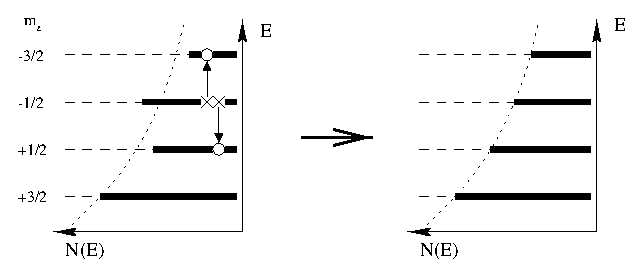
\includegraphics{drawings/relax_transition.eps}$$
	\caption[Skizze zur Einstellung des thermischen Gleichgewichts der
		Kernspins.]{{\upshape\bfseries Einstellung des thermischen Gleichgewichts der Kernspins.} Zwei
		Spins koppeln und gehen unter Erhaltung der Gesamtenergie und des Gesamtspins in einen
		jeweils anderen Zustand über.}
	\label{fig:relax_transition}
\end{figure}

Wie in Abbildung~\ref{fig:relax_transition} gezeigt koppeln die Spins ($\times$) im Niveau
$m=-\frac12$ und gehen in den Zustand ($\circ$) mit $m=-\frac32$ bzw.\ $m=\frac12$ über.
Für die Übergangsraten für diesen und den umgekehrten Prozeß gilt:
	\begin{equation}
		\left.\frac{dN}{dt}\right|_{\times\rightarrow\circ}=p_{-\frac12}p_{-\frac12}W_{\times\rightarrow\circ}\ttextt{und}
		\left.\frac{dN}{dt}\right|_{\circ\rightarrow\times}=p_{-\frac32}p_{\frac12}W_{\circ\rightarrow\times}
	\end{equation}
Im thermischen Gleichgewicht müssen diese beiden Übergangsraten übereinstimmen, da auch noch
$W_{\times\rightarrow\circ}=W_{\circ\rightarrow\times}$ gilt, erhält man:
	\begin{equation}
		\frac{p_{-\frac32}}{p_{-\frac12}}=\frac{p_{-\frac12}}{p_{+\frac12}}\quad.
	\end{equation}
Dies ist genau die Bedingung für ein thermisches Gleichgewicht nach Boltzmann, da sich die
Zustände um einen konstanten Energieabstand, also in ihrer Besetzung um einen konstanten Faktor
unterscheiden.

Man sieht, daß das thermische Gleichgewicht durch solche Prozesse erreicht wird. Die typische
Übergangsrate zwischen den Zuständen liegt in der Größenordnung der inversen Linienbreite, also bei
Metallen typischerweise in der Größenordnung von $10$ bis $100\;$µs. Falls $T_1$ viel größer als
diese Zeit zur Einstellung eines thermischen Gleichgewichts im Spinsystem ist, also z.\ B. in der
Größenordnung von Millisekunden bis Sekunden liegt, kann man die Besetzung der Kernspin"=Niveaus
als durch die Boltzmannverteilung für die Spintemperatur $T_S$ gegeben annehmen. Die Spintemperatur
stellt sich unter Erhaltung des Gesamtspins ein und kann für Tippingwinkel größer 90° aufgrund der
stärkeren Besetzung der höheren Energieniveaus auch negativ werden.

Das Spinsystem ist also durch eine Temperatur $T_S$ beschrieben, da die Besetzung der Zustände nach
\eqref{eqn:boltzmann} gegeben ist, obwohl es sich nicht im thermischen
Gleichgewicht mit einem Wärmereservoir befindet.

Die Spin"=Gitter"=Relaxation ist nun der Ausgleich des Temperaturunterschiedes zwischen der
Spintemperatur $T_S$ und der Temperatur des "`Gitters"'. Unter der Annahme, daß die
Kernspinniveaus immer einer Boltzmannverteilung genügen, kann man für die zeitliche Änderung der
inversen Spintemperatur $\beta_S=\frac1{k_BT_S}$ folgende Differentialgleichung herleiten \cite[S. 148ff]{Slichter}:
	\begin{equation}
		\frac{d\beta_S}{dt}=(\beta-\beta_S)\left[\frac12\frac{\sum_{m,n}W_{mn}(E_m-E_n)^2}{\sum_nE^2_n}\right]
			= \frac{\beta-\beta_S}{T_1}
	\end{equation}
\begin{description}
	\item[$\beta=\frac1{k_BT_\mathrm{el}}$] ist hier die inverse Temperatur des "`Gitters"'.
	\item[$W_{nm}$] stellt die Wahrscheinlichkeit für einen vom Gitter induzierten Übergang des
		Systems von Zustand $m$ in den Zustand $n$ dar.
\end{description}
Für die Relaxationszeit $T_1$ ergibt sich somit allgemein:
	\begin{equation}
		\label{eqn:t1}
		\frac1{T_1}=\frac12\frac{\sum_{m,n}W_{mn}(E_m-E_n)^2}{\sum_nE^2_n}
	\end{equation}

\subsection{Spin"=Gitter"=Relaxation der Kerne in einem Metall}

Der dominante Mechanismus der Spin"=Gitter"=Relaxation der Kerne in einem Metall ist die Kopplung an
die spin"=magnetischen Momente der Leitungselektronen.

In einem solchen $T_1$"=Prozeß gibt der Kern entweder Energie ab oder nimmt sie auf. Da die
Gesamtenergie von Gitter und Spinsystem erhalten bleibt, muß das Gitter (also das Wärmebad) dies
kompensieren. Die Kopplung an die Leitungselektronen kann man sich als einen gekoppelten Übergang
eines Kerns und eines Leitungselektrons mit Wellenvektor $\vec k$ und Spin"=Orientierung
$s$ zum Zustand $\vec k', s'$ als eine Art Streuprozeß vorstellen. Wenn man die Start"=
und Ziel"=Quantenzahlen mit $m$ und $n$ bezeichnet, erhält man für die Anzahl der Übergänge pro
Sekunde vom Startzustand $|m\vec ks>$ von Kern und Elektron zum Zielzustand $|n\vec k's'>$:
	\begin{equation}
		W_{m\vec ks, n\vec k's'}=
			\frac{2\pi}{\hbar}\abs{<m\vec ks|V|n\vec k's'>}^2\delta(E_m+E_{\vec ks}-E_n-E_{\vec k's'})
	\end{equation}
Wobei $V$ die Streu"=Wechselwirkung darstellt und angenommen wird, daß ein Elektron im Zustand
$|\vec ks>$ existiert und der Zustand $|\vec k's'>$ unbesetzt ist. Die Gesamtwahrscheinlichkeit
pro Sekunde für einen Übergang erhält man durch Summation über alle möglichen $W_{m\vec ks, n\vec
k's'}$
	\begin{equation}
		W_{mn}=\sum_{\vec k s \text{ besetzt}\atop\vec k's'\text{ unbesetzt}}W_{m\vec ks, n\vec k's'}\ttext{.}
	\end{equation}
Nun geht man zur Fermi"=Funktion $f(E_{\vec ks})$ als Verteilungsfunktion der Elektronen über und
setzt als Hauptbeitrag zur Streu"=Wechselwirkung $V$ die Kopplung der $s$"=Wellenfunktionen der
Elektronen an die Kerne an:
	\begin{equation}
		V=\frac{8\pi}{3}\gamma_e\gamma_n\;\hbar^2\vec I\cdot\vec S\,\delta(\vec r)
	\end{equation}
Hierbei nimmt man an, das sich der Kern am Ursprung des Koordinatensystems befindet und nur
Elektronen, die sich am Kernort befinden durch die Fermi"=Kontakt"=Wechselwirkung einen
Beitrag liefern.

Wenn man für die Wellenfunktion der Elektronen im Gitter das Produkt einer Spin"=Funktion und einer
Bloch"=Funktion $u_{\vec k}(\vec r)e^{i\vec k\cdot\vec r}$ ansetzt, kann man die Matrixelemente der
Streu"=Wechselwirkung berechnen. Die Summation über die Elektronenzustände kann man mit Hilfe der
Zustandsdichte $g(E_{\vec k})$ zu einer Integration über die Energie umformen. Zum Schluß ist noch
die Tatsache wichtig, daß nur Elektronen nahe der Fermi"=Kante an solchen Streuprozessen beteiligt
sein können, da die Energie, die zwischen Kern und Elektron ausgetauscht wird, im Falle hoher
Temperaturen viel kleiner als $k_BT$ ist und nur in der Nähe der Fermi"=Kante freie Zustände in
diesem Energieabstand erreicht werden können. Da die Anzahl der Elektronen in der Nähe der
Fermikante proportional zu $k_BT$ ist, folgt diese Proportionalität auch für $W_{mn}$.

Wenn man nun das berechnete $W_{mn}$ in die Gleichung \eqref{eqn:t1} einsetzt und noch über die
Anzahl $N$ der Kerne im Gitter summiert, erhält man die Korringa"=Relation \cite{Korringa}:
\begin{equation}
	\label{eqn:korringa}
	T_1\left(\frac{\Delta H}{H}\right)^2=\frac{\hbar}{4\pi k_BT_\mathrm{el}}\frac{\gamma_e^2}{\gamma_n^2}
\end{equation}
Wobei der Term $\frac{\Delta H}{H}$ die Größe der im folgenden Abschnitt erklärten Knightshift
nach \eqref{eqn:knightshift} darstellt. Die Korringarelation bestimmt das Verhältnis
von Spin"=Gitter Relaxationzeit $T_1$ , Knightshift $\frac{\Delta H}{H}$ und der
Elektronentemperatur $T_\mathrm{el}$.

%%%%%%%%%%%%%%%%%%%%%%%%%%%%%%%%%%%%%%%%%%%%%%%%%%%%%%%%%%%%%%%%%%%%%%%%%%%%%%%%%%%%%%%%%%%%%%%%%%

\section{Frequenzverschiebung in Metallen --- Knightshift}
Entdeckt wurde die Knightshift aufgrund der Verschiebung der Resonanzfrequenz in $^{63}$Cu. Da
diese Verschiebung mit 0.23\% höher ist als bekannte chemische Verschiebungen verschiedener
diamagnetischer Komponenten, suchte man den zugrundeliegenden Effekt im Metall. Darauffolgende
Untersuchungen zeigten, das dieses Phänomen in allen Metallen auftritt. Wenn man
$\omega_\mathrm{M}$ für die Resonanzfrequenz und $\omega_\mathrm{D}$ für die Resonanzfrequenz in
einer diamagnetischen Referenzumgebung schreibt, ist die Frequenzverschiebung $\Delta\omega$ bei dem
selben statischen Magnetfeld durch $\omega_\mathrm{M} = \omega_\mathrm{D} + \Delta\omega$
mit folgenden Eigenschaften gegeben:
	\begin{enumerate}
		\item $\Delta\omega$ ist im Allgemeinen positiv.
		\item Die relative Verschiebung $\frac{\Delta\omega}{\omega_\mathrm{D}}$ bleibt bei
			veränderlicher Stärke des stationären Magnetfeldes konstant.
		\item Die relative Verschiebung $\frac{\Delta\omega}{\omega_\mathrm{D}}$ ist annähernd
			temperaturunabhängig.
		\item Die relative Verschiebung nimmt im Allgemeinen mit steigender Kernladungszahl $Z$
			ab.
	\end{enumerate}

Diese zusätzliche Verschiebung der Resonanzfrequenz in Metallen folgt analog zur
Spin"=Gitter"=Relaxation aus der Kopplung der Elektronenwellenfunktionen mit $s$"=Charakter an die
Kernspins. Die Polarisation der Elektronen hängt nur vom äußeren Magnetfeld $B_0$ ab, da der
Spin"=Paramagnetismus des stark entarteten Elektronengases der Leitungselektronen unabhängig von
der Temperatur ist. Die Verschiebung $\Delta\omega$ ist also temperaturunabhängig. Die
Abhängigkeit der Verschiebung von der Kernladungszahl ist durch die bekannte, mit steigendem $Z$
größer werdende Hyperfeinaufspaltung freier Atome erklärt.

Diese Kopplung hat in Metallen, obwohl sie durch den gleichen Hamiltonian wie in Nichtmetallen
beschrieben wird, einige Besonderheiten, die aus folgenden Eigenschaften der Leitungselektronen
herrühren:

 \begin{enumerate}
	\item Die Leitungselektronen sind nicht lokalisiert. Ein bestimmtes Leitungselektron, daß nach
		dem Bloch"=Theorem durch die Wellenfunktion $\phi_{\vec k}(\vec r)=u_{\vec k}(\vec
		r)e^{i\vec k\cdot\vec r}$ beschrieben ist (mit $u_{\vec k}(\vec r)$ periodisch im
		Kristallgitter und im Volumen $V$ der Probe normiert), besitzt in der Nähe jedes Kernspins
		im Gitter die gleiche Aufenthaltswahrscheinlichkeit. Analog sieht jeder Kernspin
		gleichzeitig die Magnetfelder aller Leitungselektronen des Metalls.
	\item Für die Größenordnung der Elektronendichten $N$, die in Metallen vorkommen, verhalten
		sich die Leitungselektronen sogar bei Raumtemperatur wie ein entartetes Fermi"=Gas. In
		Anwesenheit eines Magnetfeldes $H$ sind alle Energieniveaus, außer denen in der Nähe
		der Fermi"=Energie, mit zwei Elektronen entgegengesetzten Spins aufgefüllt. Die paramagnetische Suszeptibilität
		der Leitungselektronen $\chi_e^s$ ist deshalb im Gegensatz zu der der gebundenen
		Elektronen nahezu temperaturunabhängig.
 \end{enumerate}

Wenn man zur Vereinfachung annimmt, daß das Bahnmoment der Elektronen komplett ausgelöscht ist,
erhält man die Kopplung eines gegebenen Kernspins $I$ mit den Elektronen durch Summation der
Erwartungswerte der Hyperfeinkopplungen dieses Kernspins mit allen Leitungselektronen.

Der Kernspin $\vec I$ sieht ein internes Feld $\Delta H$, das das angelegte Feld $H_0$
überlagert und eine paramagnetische Verschiebung der Kernresonanz verursacht, die als
Knightshift\footnote{nach W. D. Knight, der diese Verschiebung 1949 als erster beobachtete}
bekannt ist \cite{KNIGHT49}.
	\begin{equation}
		\label{eqn:knightshift}
		\frac{\Delta H}{H_0}=\frac{8\pi}{3}\left<\abs{u_{\vec k}(0)}^2\right>_{E_F}\chi_e^s
	\end{equation}
